%% Copernicus Publications Manuscript Preparation Template for LaTeX Submissions
%% ---------------------------------
%% This template should be used for the following class files: copernicus.cls, copernicus2.cls, copernicus_discussions.cls
%% The class files, the Copernicus LaTeX Manual with detailed explanations regarding the comments
%% and some style files are bundled in the Copernicus Latex Package which can be downloaded from the different journal webpages.
%% For further assistance please contact the Publication Production Office (production@copernicus.org).
%% http://publications.copernicus.org


%% Differing commands regarding the specific class files are highlighted.


%% copernicus.cls
\documentclass[gmd]{copernicus}

\begin{document}

\linenumbers

\title{MicroHH 1.0: a computational fluid dynamics code for direct and large-eddy simulation of atmospheric boundary layer flows}


\author[1]{Chiel C. van Heerwaarden}
\author[1]{Bart J. H. van Stratum}
\author[2]{Thijs Heus}
\author[3]{Jeremy A. Gibbs}
\author[3]{Evgeni Fedorovich}

\affil[1]{Max Planck Institute for Meteorology, Hamburg, Germany}
\affil[2]{Cleveland State University, Cleveland, OH, USA}
\affil[3]{University of Oklahoma, Norman, OK, USA}

%% The [] brackets identify the author to the corresponding affiliation, 1, 2, 3, etc. should be inserted.



\runningtitle{MicroHH 1.0}

\runningauthor{van Heerwaarden et al.}

\correspondence{Chiel van Heerwaarden\\ (chiel.vanheerwaarden@mpimet.mpg.de)}



\received{}
\pubdiscuss{} %% only important for two-stage journals
\revised{}
\accepted{}
\published{}

%% These dates will be inserted by the Publication Production Office during the typesetting process.


\firstpage{1}

\maketitle  %% Please note that for the copernicus2.cls this command needs to be inserted after \abstract{TEXT}

\begin{abstract}
This paper describes MicroHH 1.0, a new Computational Fluid Dynamical code for the simulation of wall-bounded turbulent flows in the atmosphere using Direct Numerical Simulation and Large-Eddy Simulation. The paper covers the description of the governing equations, their numerical implementation and the parametrizations involved in the code. Furthermore, the paper presents the validation of the dynamical core in the form of convergence tests and conservation tests and comparison of simulations of channel flows and slope flows against well-established models. The full numerical model, including the associated parametrizations for Large-Eddy simulations of high Reynolds number flows, has been tested for a set of cases under stable and unstable conditions, under the Boussinesq and anelastic approximation and with dry and moist convection under stationary and time-varying boundary conditions. The paper presents performance tests showing good scaling from 256 to 32,738 processes. The GPU version of the code reaches speedups of more than an order of magnitude with respect to the conventional CPU code for a variety of cases.
\end{abstract}

\introduction  %% \introduction[modified heading if necessary]
In this paper we present a description of MicroHH 1.0, a new Computational Fluid Dynamical code for the simulation of wall-bounded turbulent flows, with a focus on those in the atmosphere. MicroHH is a model that can be run both for Direct Numerical Simulations as well as for Large-Eddy Simulations with applications ranging from channel flows to cloudy boundary layers. The model has been designed and written from scratch with the aim of creating a highly parallel code that is able to run on more than 10,000 processes with the support of modern techniques. MicroHH has been written in C++, in contrast to the majority of its peers, which are written in Fortran 90. The reasons we explain in Section \ref{sec:technical}.

In this paper we provide a full description of the governing equations and their numerical implementation. In addition, we discuss the added parametrizations and their underlying assumptions.

\section{Dynamical core: governing equations}
The dynamical core of MicroHH follows the conservation equations under the anelastic approximation as shown in BANNON1996. The approximation directly simplifies to the Boussinesq equations if the base density $\rho_0$ is assumed to be constant with height.

\subsection{Conservation of mass}
The conservation of mass is formulated as:
\begin{eqnarray}
\dfrac{\partial \rho_0 u_i}{\partial x_i} & = & 0\label{eq:consmassa}.
\end{eqnarray}

Under the Boussinesq approximation, the equation simplifies to conservation of volume:
\begin{eqnarray}
\dfrac{\partial u_i}{\partial x_i} & = & 0\label{eq:consmassb}
\end{eqnarray}

\subsection{Conservation of momentum}
The momentum equation is written it the flux form, in order to assure the best possible mass and momentum conservation. The hydrostatic balance $dp_0 / dz~=~-\rho_0 g$ has been subtracted to arrive at the perturbation form:
\begin{eqnarray}
\dfrac{\partial u_i}{\partial t} & = & - \dfrac{1}{\rho_0} \dfrac{\partial \rho_0 u_i u_j}{\partial x_j} 
- \dfrac{\partial}{\partial x_i}\left(\dfrac{p'}{\rho_0}\right) + g \dfrac{\theta_v'}{\theta_{v0}} + \nu \dfrac{\partial^2 u_i}{\partial x_j^2}\label{eq:consmoma},\\
\dfrac{\theta_v'}{\theta_{v0}} & = & \dfrac{p'}{\rho g H_{\rho}} - \dfrac{\rho'}{\rho_0}\label{eq:statea},
\end{eqnarray}
where the scale height of density is defined as: $H_{\rho}~\equiv~\left( \dfrac{1}{\rho_0} \dfrac{d\rho_0}{dz} \right)^{-1}$. Under the Boussinesq approximation, where $\rho_0$ is constant with height and the scale height for density $H_\rho$ approaches infinity, the set simplifies to:
\begin{eqnarray}
\dfrac{\partial u_i}{\partial t} & = & - \dfrac{\partial u_i u_j}{\partial x_j}
- \dfrac{1}{\rho_0}\dfrac{\partial p}{\partial x_i} + g \dfrac{\theta_v'}{\theta_{v0}} + \nu \dfrac{\partial^2 u_i}{\partial x_j^2}\label{eq:consmomb},\\
\dfrac{\theta_v'}{\theta_{v0}} & = & - \dfrac{\rho'}{\rho_0}\label{eq:stateb}.
\end{eqnarray}

\subsection{Pressure equation}
For simplicity we define function $f$ that contains all right hand side terms of Eq., except the pressure gradient. In order to arrive at the equation that allows us to solve for the pressure we multiply the equation with the base density $\rho_0$ and take the divergence. Conservation of mass ensures that the tendency term vanishes, such that an elliptic equation remains for the pressure:
\begin{eqnarray}
\dfrac{\partial}{\partial x_i} 
\left[ \rho_0 \dfrac{\partial}{\partial x_i} \left( \dfrac{p'}{\rho_0} \right) \right] & = &
\dfrac{\partial \rho_0 f_i}{\partial x_i}.
\end{eqnarray}
Under the Boussinesq approximation the equation simplifies to:
\begin{eqnarray}
\label{eq:poisson}
\dfrac{\partial^2}{\partial x_i^2} \left( \dfrac{p'}{\rho_0} \right) & = &
\dfrac{\partial f_i}{\partial x_i}.
\end{eqnarray}


\subsection{Conservation of an arbitrary scalar}
The conservation equation of an arbitrary scalar $\phi$ can be written in flux form:
\begin{eqnarray}
\dfrac{\partial \phi}{\partial t} & = & - \dfrac{1}{\rho_0} \dfrac{\partial \rho_0 u_j \phi}{\partial x_j} +
\kappa_\phi \dfrac{\partial^2 \phi}{\partial x_j^2} + S_\phi,
\end{eqnarray}
where $S_\phi$ represents sources and sinks of the variable.

\subsection{Conservation of energy}
MicroHH supports a series of governing equations for the energy equation. In short there are two modes, one that uses the potential temperature as a prognostic variable
\begin{eqnarray}
\dfrac{\partial \theta}{\partial t} & = & - \dfrac{1}{\rho_0} \dfrac{\partial \rho_0 u_j \theta}{\partial x_j} + \kappa_\phi \dfrac{\partial^2 \theta}{\partial x_j^2} + \dfrac{\theta_0}{\rho_0 c_p T_0} Q,
\end{eqnarray}
and one that uses the liquid water potential temperature $\theta_l$.



\subsection{Simplification of the Boussinesq system and the extension to slope flows}
Under the Boussinesq approximation with only dry thermodynamics ($\theta_v = \theta$), the equation of state can be eliminated and the conservation of momentum and energy can be written as:
\begin{eqnarray}
\dfrac{\partial u_i}{\partial t} + \dfrac{\partial u_i u_j}{\partial x_j} & = & 
- \dfrac{1}{\rho_0}\dfrac{\partial p'}{\partial x_i} + \delta_{i3} b + \nu \dfrac{\partial^2 u_i}{\partial x_j^2}\label{eq:consmombsimp},\\
\dfrac{\partial b}{\partial t} + \dfrac{\partial b u_j}{\partial x_j} & = & 
\kappa_b \dfrac{\partial^2 b}{\partial x_j^2}\label{eq:consenbsimp}
\end{eqnarray}

With a slight modification to the previous set of equations, it is possible to study slope flows in periodic domains. If we no longer assume that gravity is directed along the z-axis, but instead assume that the domain is under a slope $\alpha$ such that gravity is distributed between the x-axis and z-axis, and assume that the reference buoyancy increases with height with slope $N^2$, the equations can be written as:
\begin{eqnarray}
\dfrac{\partial u}{\partial t} + \dfrac{\partial u_j u}{\partial x_j} & = & 
- \dfrac{1}{\rho_0}\dfrac{\partial p'}{\partial x} + \sin(\alpha) b + \nu \dfrac{\partial^2 u}{\partial x_j^2}\label{eq:consuslope},\\
\dfrac{\partial w}{\partial t} + \dfrac{\partial u_j w}{\partial x_j} & = & 
- \dfrac{1}{\rho_0}\dfrac{\partial p'}{\partial z} + \cos(\alpha) b + \nu \dfrac{\partial^2 w}{\partial x_j^2}\label{eq:conswslope},\\
\dfrac{\partial b}{\partial t} + \dfrac{\partial b u_j}{\partial x_j} & = & 
\kappa_b \dfrac{\partial^2 b}{\partial x_j^2} - \left (u\,\sin(\alpha) + w\,\cos(\alpha) \right) N^2\label{eq:consbslope}
\end{eqnarray}

\section{Dynamical core: numerical implementation}
\subsection{Time integration}
The prognostic equations are solved using low-storage Runge-Kutta time integration schemes, where each prognostic variable requires only two three dimensional fields. The code provides two options: a three-stage third order scheme (WILSON) and a five stage fourth order scheme (CARPENTER). Both of them can be written in the same general form in semi-discrete formulation:
\begin{eqnarray}
f\left(\phi^n\right) & = & a^n f\left( \phi^{n-1} \right) \\
\phi^{n+1} & = & \phi^n + b^n \Delta t f\left(\phi^n\right),
\end{eqnarray}
where $f$ is a function that represent the computation of all right hand side terms, $\phi$ is an arbitrary variable and $a$ and $b$ are the coefficients for the Runge-Kutta method at stage $n$. In principle, in low storage form, the tendencies of the previous stage $n-1$ are retained and multiplied with $a^n$ at the beginning of a stage, except for the first stage, where $a_1 = 0$. During the time integration, the tendency is multiplied with coefficient $b^n$ in order to find the value of arbitrary variable $\phi$ in stage $n+1$.

For the third-order scheme the vectors $a$ and $b$ are:
\begin{eqnarray}
a & = & \left\{0, -\frac{5}{9}, -\frac{153}{128} \right\}\\
b & = & \left\{\frac{1}{3}, \frac{15}{16}, \frac{8}{15} \right\}
\end{eqnarray}

For the fourth-order scheme the vectors $a$ and $b$ are:
\begin{eqnarray}
\nonumber a & = & \left\{0, -\frac{567301805773}{1357537059087},
-\frac{2404267990393}{2016746695238},\right.\\
& & \left. -\frac{3550918686646}{2091501179385},
-\frac{1275806237668}{842570457699} \right\}\\
\nonumber b & = & \left\{\frac{1432997174477}{9575080441755}, \frac{5161836677717}{13612068292357},
\frac{1720146321549}{2090206949498},\right.\\
& & \left. \frac{3134564353537}{4481467310338},
\frac{2277821191437}{14882151754819} \right\}
\end{eqnarray}

Even though the fourth order scheme has five stages and is thus considerably more expensive than the third order scheme, the truncation error is so much smaller that under many conditions it pays off to use fourth order scheme. We demonstrate this in Section \ref{sec:validationtime}, where we study the conservation properties of the model and the accuracy of the time integration scheme.

\subsection{Grid}
MicroHH is discretized on a staggered grid, where the scalars are located in the center of a grid cell and the three velocity components at the faces.

MicroHH can work with stretched grids in the vertical dimension. The grid is initialized from vertical profiles that give the location of the cell centres. The locations of the faces are determined consistent with the spatial order of the interpolations that are described in the next section.

\subsection{Building blocks of the spatial discretization}
The spatial operators are based on finite differences. The code supports second order and fourth order accurate discretizations, which follow \citet{Morinishi1998, Vasilyev2000}. From Taylor series spatial operators can be derived that form the building blocks of more advanced operators, such as the advection and diffusion operators. In the following section we describe for simplicity the operators and the derived operators in two dimensions.

First, there are the second order accurate interpolation operators:
\begin{eqnarray}
\phi_{i,j} \approx \widehat{\phi}^{2x }_{i,j} & \equiv & \dfrac{\phi_{i-\frac{1}{2},j} + \phi_{i+\frac{1}{2},j}}{2},\\
\phi_{i,j} \approx \widehat{\phi}^{2xL}_{i,j} & \equiv & \dfrac{\phi_{i-\frac{3}{2},j} + \phi_{i+\frac{3}{2},j}}{2},
\end{eqnarray}
and the gradient operators defined using the same stencil size:
\begin{eqnarray}
\left. \dfrac{\partial \phi}{\partial x}\right|_{i,j} \approx \delta^{2x} \left( \phi \right)_{i,j} & \equiv & \dfrac{\phi_{i+\frac{1}{2},j} - \phi_{i-\frac{1}{2},j}}
                                                                                                                 {   x_{i+\frac{1}{2}}   -    x_{i-\frac{1}{2}  }} \\
\left. \dfrac{\partial \phi}{\partial x}\right|_{i,j} \approx \delta^{2xL} \left( \phi \right)_{i,j}& \equiv & \dfrac{\phi_{i+\frac{3}{2},j} - \phi_{i-\frac{3}{2},j}}
                                                                                                                  {   x_{i+\frac{3}{2}}   -    x_{i-\frac{3}{2}  }}
\end{eqnarray}
In our notation, we use the Einstein summation in the operators. For instance, the divergence of vector $\left.u_i\right|_{i,j}$ can be written as $\delta^{2x_i}\left( u_i \right)$.
% \begin{eqnarray}
% \delta^{2x} \left( \phi \right)_{i,j} = \dfrac{\phi_{i+\frac{1}{2},j} - \phi_{i-\frac{1}{2},j}}
%                                               {\Delta x}
% \end{eqnarray}
% 
% \begin{eqnarray}
% \delta^{2xL} \left( \phi \right)_{i,j} = \dfrac{\phi_{i+\frac{3}{2},j} - \phi_{i-\frac{3}{2},j}}
%                                                {3\Delta x}
% \end{eqnarray}

\subsubsection{Fourth-order operators}
Similar to the second-order operators, also fourth-order ones can be defined:
\begin{eqnarray}
\phi_{i,j} \approx \widehat{\phi}^{4x}_{i,j} \equiv \dfrac{- \phi_{i-\frac{3}{2},j} + 9 \phi_{i-\frac{1}{2},j} + 9 \phi_{i+\frac{1}{2},j} - \phi_{i+\frac{3}{2},j}}{16},\label{eq:interp4}
\end{eqnarray}
and a biased one that can by applied in the vicinity of the boundaries:
\begin{eqnarray}
\phi_{i,j} \approx \widehat{\phi}^{4xb}_{i,j} \equiv \dfrac{ 5 \phi_{i-\frac{1}{2},j} + 15 \phi_{i+\frac{1}{2},j} - 5 \phi_{i+\frac{3}{2},j} + \phi_{i+\frac{5}{2},j}}{16}.
\end{eqnarray}

For these stencils the gradient operators are:
\begin{eqnarray}
\nonumber
\left. \dfrac{\partial \phi}{\partial x}\right|_{i,j} & \approx & \delta^{4x} \left( \phi \right)_{i,j}\\
& \equiv & \dfrac{\phi_{i-\frac{3}{2},j} - 27 \phi_{i-\frac{1}{2},j} + 27 \phi_{i+\frac{1}{2},j} - \phi_{i+\frac{3}{2},j}}
             {       x_{i-\frac{3}{2}}   - 27    x_{i-\frac{1}{2}}   + 27    x_{i+\frac{1}{2}}   -    x_{i+\frac{3}{2}}},
\end{eqnarray}
and

\begin{eqnarray}
\nonumber
\left. \dfrac{\partial \phi}{\partial x}\right|_{i,j} & \approx & \delta^{4xb} \left( \phi \right)_{i,j}\\
& \equiv & \dfrac{-23 \phi_{i-\frac{1}{2},j} + 21 \phi_{i+\frac{1}{2},j} + 3 \phi_{i+\frac{3}{2},j} - \phi_{i+\frac{5}{2},j}}
                 {-23    x_{i-\frac{1}{2}}   + 21    x_{i+\frac{1}{2}}   + 3    x_{i+\frac{3}{2}}   -    x_{i+\frac{5}{2}}}
\end{eqnarray}

% \begin{eqnarray}
% \delta^{4x} \left( \phi \right)_{i,j}  = \dfrac{\phi_{i-\frac{3}{2},j} - 27 \phi_{i-\frac{1}{2},j} + 27 \phi_{i+\frac{1}{2},j} - \phi_{i+\frac{3}{2},j}}
%                                                {24 \Delta x}
% \end{eqnarray}

% \begin{eqnarray}
% \nonumber 
% &&\left. \dfrac{\partial^2 \phi}{\partial x^2}\right|_{i,j} \approx \delta^{4x} \left( \delta^{4x} \left( \phi \right) \right)_{i,j}\\
% \nonumber
% && = \dfrac{1}{576 \left( \Delta x \right)^2} \left( \phi_{i-3,j} - 54 \phi_{i-2,j} + 783 \phi_{i-1,j}\right.\\
% &&  \left. - 1460  \phi_{i,j} + 783 \phi_{i+1,j} - 54 \phi_{i+2,j} + \phi_{i+3,j} \right)
% \end{eqnarray}

\subsection{Advection}
The advection term is discretized in the flux form:
\begin{eqnarray}
\nonumber
\dfrac{\partial u \phi}{\partial x} + \dfrac{\partial v \phi}{\partial y} & \approx & 
\delta^{2x} \left( u \widehat{\phi}^{2x} \right)_{i,j} + \delta^{2y} \left( u \widehat{\phi}^{2y} \right)_{i,j} \\ 
& = & \dfrac{ u_{i+\frac{1}{2},j} \widehat{\phi}^{2x}_{i+\frac{1}{2},j} - u_{i-\frac{1}{2},j} \widehat{\phi}^{2x}_{i-\frac{1}{2},j} }
            { x_{i+\frac{1}{2}} - x_{i-\frac{1}{2}} }\\
& + & \dfrac{ v_{i,j+\frac{1}{2}} \widehat{\phi}^{2y}_{i,j+\frac{1}{2}} - v_{i,j-\frac{1}{2}} \widehat{\phi}^{2y}_{i,j-\frac{1}{2}} }
            { y_{j+\frac{1}{2}} - y_{j-\frac{1}{2}} }
\end{eqnarray}

\begin{eqnarray}
\dfrac{\partial v u}{\partial x} = \delta^{2x} \left( \widehat{v}^{2y} \widehat{u}^{2x} \right)_{i,j} =
\dfrac{ \widehat{v}^{2y}_{i+\frac{1}{2},j} \widehat{u}^{2x}_{i+\frac{1}{2},j} - \widehat{v}^{2y}_{i-\frac{1}{2},j} \widehat{u}^{2x}_{i-\frac{1}{2},j} }
      { x_{i+\frac{1}{2}} - x_{i-\frac{1}{2}} }\label{eq:advec2u}
\end{eqnarray}
In the standard fourth-order scheme:
\begin{eqnarray}
\nonumber
\left. \dfrac{\partial u \phi}{\partial x} \right|_{i,j} & \approx & \delta^{4x} \left( u \widehat{\phi}^{4x} \right)_{i,j} \\
\nonumber
& = & \left( u_{i-\frac{3}{2},j} \widehat{\phi}^{4x}_{i-\frac{3}{2},j} - 27 u_{i-\frac{1}{2},j} \widehat{\phi}^{4x}_{i-\frac{1}{2},j} \right.\\
\nonumber
&   &\left. + 27 u_{i+\frac{1}{2},j} \widehat{\phi}^{4x}_{i+\frac{1}{2},j} - u_{i+\frac{3}{2},j} \widehat{\phi}^{4x}_{i+\frac{3}{2},j} \right)\\
&   &\slash \left( x_{i-\frac{3}{2}} - 27 x_{i-\frac{1}{2}} + 27 x_{i+\frac{1}{2}} - x_{i+\frac{3}{2}} \right)
\end{eqnarray}
Hereafter, we assume that the usage of the operators is clear and we no longer expand them.

The fully energy conserving scheme is an interpolation of two second order operators:
\begin{eqnarray}
% \nonumber
\left. \dfrac{\partial u \phi}{\partial x} \right|_{i,j} & = & \frac{9}{8} \delta^{2x} \left( u \widehat{\phi}^{2x} \right)_{i,j} 
                                                             - \frac{1}{8} \delta^{2xL} \left( u \widehat{\phi}^{2xL} \right)_{i,j}%\\
% \nonumber
% & = & \frac{9}{16} \dfrac{ u_{i+\frac{1}{2},j} \widehat{\phi}^x_{i+\frac{1}{2},j} - u_{i-\frac{1}{2},j} \widehat{\phi}^x_{i-\frac{1}{2},j} }
%                           { x_{i+\frac{1}{2}} - x_{i-\frac{1}{2}} }\\
% & - & \frac{1}{16} \dfrac{ u_{i+\frac{3}{2},j} \widehat{\phi}^{3x}_{i+\frac{3}{2},j} - u_{i-\frac{3}{2},j} \widehat{\phi}^{3x}_{i-\frac{3}{2},j} }
%                           { x_{i+\frac{3}{2}} - x_{i-\frac{3}{2}} }
\end{eqnarray}
Note that in this scheme velocity interpolations, such as in Eq. \ref{eq:advec2u}, still need to be performed with fourth order accuracy (Eq. \ref{eq:interp4}) in order to keep the total operator fourth order accurate. Therefore, for instance:
\begin{eqnarray}
\dfrac{\partial v u}{\partial x} \approx \frac{9}{8} \delta^{2x} \left( \widehat{v}^{4y} \widehat{u}^{2x} \right)_{i,j} 
                                       - \frac{1}{8} \delta^{2xL} \left( \widehat{v}^{4y} \widehat{u}^{2xL} \right)_{i,j}
\end{eqnarray}

\subsection{Diffusion}
The diffusion operator is calculated as a divergence of a gradient:
\begin{eqnarray}
\left. \kappa_\phi \dfrac{\partial^2 \phi}{\partial x^2}\right|_{i,j} & \approx &
\kappa_\phi \delta^{2x} \left( \delta^{2x} \left( \phi \right) \right)_{i,j}\\
% \kappa_\phi \dfrac{\left. \dfrac{\partial \phi}{\partial x}\right|_{i+\frac{1}{2},j} - \left. \dfrac{\partial \phi}{\partial x}\right|_{i-\frac{1}{2},j}}
%                                 {   x_{i+\frac{1}{2},j} -    x_{i-\frac{1}{2},j}}
\left. \kappa_\phi \dfrac{\partial^2 \phi}{\partial x^2}\right|_{i,j} & \approx &
\kappa_\phi \delta^{4x} \left( \delta^{4x} \left( \phi \right) \right)_{i,j}
\end{eqnarray}
On an equidistant grid, this leads to the well-known second order accurate operator for the second derivate:
\begin{eqnarray}
\kappa_\phi \delta^{2x} \left( \delta^{2x} \left( \phi \right) \right)_{i,j} =
\kappa_\phi \dfrac{ \phi_{i-1,j} - 2 \phi_{i,j} + \phi_{i+1,j} }{\left( \Delta x \right)^2},
\end{eqnarray}
whereas for a fourth-order accurate operator, a seven-point stencil is derived:
\begin{eqnarray}
\nonumber
&& \kappa_\phi \delta^{4x} \left( \delta^{4x} \left( \phi \right) \right)_{i,j}\\
\nonumber
&& = \dfrac{\kappa_\phi}{576 \left( \Delta x \right)^2} \left( \phi_{i-3,j} - 54 \phi_{i-2,j} + 783 \phi_{i-1,j}\right.\\
&&  \left. - 1460  \phi_{i,j} + 783 \phi_{i+1,j} - 54 \phi_{i+2,j} + \phi_{i+3,j} \right)
\end{eqnarray}

% \begin{eqnarray}
% \nonumber
% \left. \kappa_\phi \dfrac{\partial^2 \phi}{\partial x^2}\right|_{i,j} & = & \kappa_\phi
% \left( \left. \dfrac{\partial \phi}{\partial x}\right|_{i-\frac{3}{2},j} 
% - 27 \left. \dfrac{\partial \phi}{\partial x}\right|_{i-\frac{1}{2},j} \right. \\
% \nonumber
% & & \left. + 27 \left. \dfrac{\partial \phi}{\partial x}\right|_{i+\frac{1}{2},j} 
% - \left. \dfrac{\partial \phi}{\partial x}\right|_{i+\frac{3}{2},j} \right)\\
% & & / \left( x_{i-\frac{3}{2}} - 27    x_{i-\frac{1}{2}} + 27    x_{i+\frac{1}{2}} -    x_{i+\frac{3}{2}} \right)
% \end{eqnarray}
\subsection{Pressure}
The pressure solver follows the method of Chorin19XX.
Modified wavenumber
\begin{eqnarray}
\left. \widetilde{u_i} \right|^{t+1}_{i,j,k} & = & \left. u_i \right|^{t}_{i,j,k} + \Delta t \left. f_i \right|^{t}_{i,j,k}\\
\left. u_i\right|^{t+1}_{i,j,k} & = & \left. \widetilde{u_i} \right|^{t+1}_{i,j,k} - \Delta t \left. \delta^{nx_i}\left( \dfrac{p}{\rho_0}\right)\right|^t_{i,j,k}
\end{eqnarray}
\begin{eqnarray}
\left. \delta^{nx_i} \left( \rho_0 u_i\right) \right|^{t+1}_{i,j,k} & = & 
\left. \delta^{nx_i} \left( \rho_0 \widetilde{u_i} \right) \right|^{t+1}_{i,j,k}\\
& - &  \Delta t \left.\delta^{nx_i} \left[ \rho_0 \delta^{nx_i}\left( \dfrac{p}{\rho_0}\right) \right] \right|^t_{i,j,k}
\end{eqnarray}
We set the left hand side to zero, to enforce a divergence free field at the next time step, which leaves us with the Poisson equation:
\begin{eqnarray}
\dfrac{\left. \delta^{nx_i} \left( \rho_0 \widetilde{u_i} \right) \right|^{t+1}_{i,j,k}}{\Delta t}
& = &  \left. \delta^{nx_i} \left[ \rho_0 \delta^{nx_i}\left( \dfrac{p}{\rho_0}\right) \right] \right|^t_{i,j,k},
\end{eqnarray}
which is the discretized version of Eq. \ref{eq:poisson}

In order to simplify the notation, we name the left hand side term $\psi$ and the $p / \rho_0$ term on the right hand side $\pi$. Solving a Poisson equation is a global operation. Since the fields are periodic in the horizontal directions on an equidistant grid and the function is linear, we can perform a Fourier transform in the two horizontal directions:
\begin{eqnarray}
\widehat{\psi}_{l,m,k} = - k^2_{*n} \widehat{\pi}_{l,m,k} - l^2_{*n} \widehat{\pi}_{l,m,k}
+ \delta^{nz} \left[ \rho_0 \delta^{nz} \left( \widehat{\pi} \right) \right]_{l,m,k},
\end{eqnarray}
where $k_*$ and $l_*$ are the squares of the modified wave numbers belonging to the discretization:
\begin{eqnarray}
-k_{*2}^2 & \equiv & 2 \dfrac{\cos (k \Delta x)}{\left( \Delta x \right)^2} - \dfrac{2}{\left( \Delta x \right)^2}\\
\nonumber
-k_{*4}^2 & \equiv & 2 \dfrac{\cos (3k \Delta x) - 54 \cos (2k \Delta x) + 783 \cos (k \Delta x)}
{576 \left( \Delta x \right)^2}\\
& - & \dfrac{1460}{576 \left( \Delta x \right)^2}
\end{eqnarray}
The previous expressions fulfill the limit:
\begin{eqnarray}
\lim_{\Delta x \rightarrow 0} k_{*n}^2 = k^2
\end{eqnarray}

\subsection{Boundary conditions}
The lateral boundaries in MicroHH are periodic. The bottom and top boundary conditions can be formulated in their most general form, the Robin boundary condition:
\begin{eqnarray}
a \phi_s + b \left.\dfrac{\partial \phi}{\partial z}\right|_s = c,
\end{eqnarray}
which gives the Dirichlet boundary condition when ${a=1,~b=0}$ and the Neumann boundary condition when ${a=0,~b=1}$. 

MicroHH makes use of ghost cells in order to avoid the need of biased schemes for single interpolation or gradient operators near the wall. The values at the ghost cells are derived making use of the boundary conditions. 

The ghost cells for the Dirichlet boundary conditions in the second order accurate discretization are:
\begin{eqnarray}
\phi_{-\frac{1}{2}} & = & 2 c - \phi_{\frac{1}{2}},
\end{eqnarray}
whereas those for the Neumann boundary condition are:
\begin{eqnarray}
\phi_{-\frac{1}{2}} & = & -c \left( - z_{-\frac{1}{2}} + z_{\frac{1}{2}} \right) + \phi_{\frac{1}{2}}
\end{eqnarray}

In case of the fourth order scheme, we have two ghost cells and therefore a second boundary condition is required. Here we set the third order derivative equal to zero (see \citet{Morinishi1998}). For the Dirichlet boundary condition we arrive at the following expressions for the ghost cells:
\begin{eqnarray}
\phi_{-\frac{1}{2}} & = & \dfrac{8 c - 6 \phi_{\frac{1}{2}} + \phi_{\frac{3}{2}}}{3} \\
\phi_{-\frac{3}{2}} & = & 8 c - 6 \phi_{\frac{1}{2}} + \phi_{\frac{3}{2}},
\end{eqnarray}
whereas in case of a Neumann boundary condition we find:
\begin{eqnarray}
\phi_{-\frac{1}{2}} & = & -c  \dfrac{z_{i-\frac{3}{2}} - 27 z_{i-\frac{1}{2}} + 27 z_{i+\frac{1}{2}} - z_{i+\frac{3}{2}}}{24} + \phi_{\frac{1}{2}} \\
\phi_{-\frac{3}{2}} & = & -3c \dfrac{z_{i-\frac{3}{2}} - 27 z_{i-\frac{1}{2}} + 27 z_{i+\frac{1}{2}} - z_{i+\frac{3}{2}}}{24} + \phi_{\frac{3}{2}}
\end{eqnarray}

\section{Physical parametrizations}
\subsection{Surface model}
In LES mode, it is possible to make use of a surface model to calculate the appropriate surface fluxes

\begin{eqnarray}
L   & \equiv & - \dfrac{u_*^3}{\kappa B_0} \\
f_m & \equiv & \dfrac{\kappa}
  { \ln{\left( \frac{z_1}{z_{0m}} \right)}
  - \varPsi_m \left( \frac{z_1}{L} \right)
  + \varPsi_m \left( \frac{z_{0m}}{L} \right) } \\
f_h & \equiv &
  \dfrac{\kappa}
  { \ln{\left( \frac{z_1}{z_{0h}} \right)}
  - \varPsi_h \left( \frac{z_1}{L} \right)
  + \varPsi_h \left( \frac{z_{0h}}{L} \right) } \\
u_* & \equiv & f_m \left( u_1 - u_0 \right) \\
b_* & \equiv & f_h \left( b_1 - b_0 \right) 
\end{eqnarray}

MicroHH supports three different boundary conditions, each with their own bulk Richardson number.
\begin{itemize}
  \item Fixed $u_*$, fixed surface buoyancy flux $B_0$.
  \begin{equation}
    \dfrac{z}{L} = Ri_a = - \dfrac{\kappa z B_0}{u_*^3}
  \end{equation}
  
  \item Fixed surface velocity $u_0$, fixed surface buoyancy flux $B_0$.
  \begin{equation}
    \dfrac{z}{L} f_m^3 = Ri_b = - \dfrac{\kappa z B_0}{ \left(u_1 - u_0 \right)^3}
  \end{equation}
  \item Fixed surface velocity $u_0$, fixed surface buoyancy $b_0$.
  \begin{equation}
    \dfrac{z}{L} \dfrac{f_m^2}{f_h} = Ri_c = \dfrac{\kappa z \left(b_1 - b_0 \right)}{ \left(u_1 - u_0 \right)^2}
  \end{equation}
\end{itemize}

unstable $\zeta = z/L$ (Wyngaard book, Wilson):
\begin{eqnarray}
\phi_{m,h} & = & \left( 1 + \gamma_{m,h} \left| \zeta \right|^{2/3} \right)^{-1/2}\\
%\phi_h & = & \left( 1 + \gamma_h \left| z/L \right|^{2/3} \right)^{-1/2}\\
\varPsi_{m,h} & = & 3 \ln{\left( \dfrac{1 + \phi_{m,h}^{-1}}{2} \right)} 
%\Psi_m & = & \left( 1 + (3.6 \frac{z}{L})^{2/3} \right)^{-\frac{1}{2}} \\
%\Psi_h & = & \left( 1 + (3.6 \frac{z}{L})^{2/3} \right)^{-\frac{1}{2}} \\
\end{eqnarray}
where $\gamma_m = 3.6$ and $\gamma_h = 7.9$.\\
stable (Hogstrom, Wyngaard book)
\begin{eqnarray}
\phi_{m,h} & = & 1 + \lambda_{m,h} \zeta\\
\varPsi_{m,h} & = & - \lambda_{m,h} \zeta
\end{eqnarray}
where $\lambda_m = 4.8$ and $\lambda_h = 7.8$.

In all three options the function on the lefthand side has a universal shape that can be calculated a-priori and stored in a lookup table against which the respective Richardson number can be compared during the simulation to find the correct value of the stability parameter $z/L$. The lookup tables have $10^4$ entries, of which 90 percent is spaced uniformly between $z/L = -5$ to $5$. The remaining 10 percent are used to stretch the negative range up to $z/L = -10^4$ to allow for the correct free convection limit.

\subsection{Subfilter scale model}
\subsection{Thermodynamics}

\section{Technical details of the code}\label{sec:technical}
\subsection{Code structure}
MicroHH is written in C++ and makes use of aspects of object-oriented programming. The model components are written in classes, to allow for a straightforward substitution and to avoid unnecessary switch statements inside of the code. Public and protected functions inside of the classes are declared virtual to open the possibility of overriding them in a derived class. This organization of the code has the advantage that any extension or case-specific code can be put in its own file, in order to minimize the amount of code that needs to be edited and to allow for an easier merging with newer versions of the code.

The GPU version of the code is activated through preprocessor statements. 

\subsection{Parallelization}
The code uses the Message Passing Interface (MPI) in order to run on a large number of processes. The code creates a Cartesian grid using the MPI\_Cart\_create function and uses this grid to detect the IDs of neighboring processes. In order to avoid complex packing routines, we make use of MPI datatypes wherever possible. The MPI calls are written in an interface, such that the typical user never has to write any MPI calls for his personal routines.

The Input/Output (IO) is entirely based on MPI-IO, such that three dimensional fields and two dimensional cross sections are stored as single files. We have chosen for MPI-IO in order to limit the number of files written by simulations done on a large number of processes and to allow for restarts on a different number of processes. In order to keep the code as clean as possible, we make use of the MPI\_Sub\_array function in combination with MPI\_File\_write\_all in order to write three dimensional fields and cross sections.

\subsection{External dependencies}
MicroHH depends on three external software tools or libraries. First, it uses the CMake build system for the generation of Makefiles. CMake allows for parallel builds, which minimizes the compilation time. Furthermore, the FFTW3 library \citep{Frigo2005} is used for the computation of the Fast-Fourier Transforms. Last, the statistical routines save their output in NetCDF format and therefore rely on UCAR's NetCDF library. In order to run the provided test cases and their output scripts a Python installation including the Pylab library is required.

\section{Scaling experiments}
\begin{figure}[t]
\vspace*{2mm}
\begin{center}
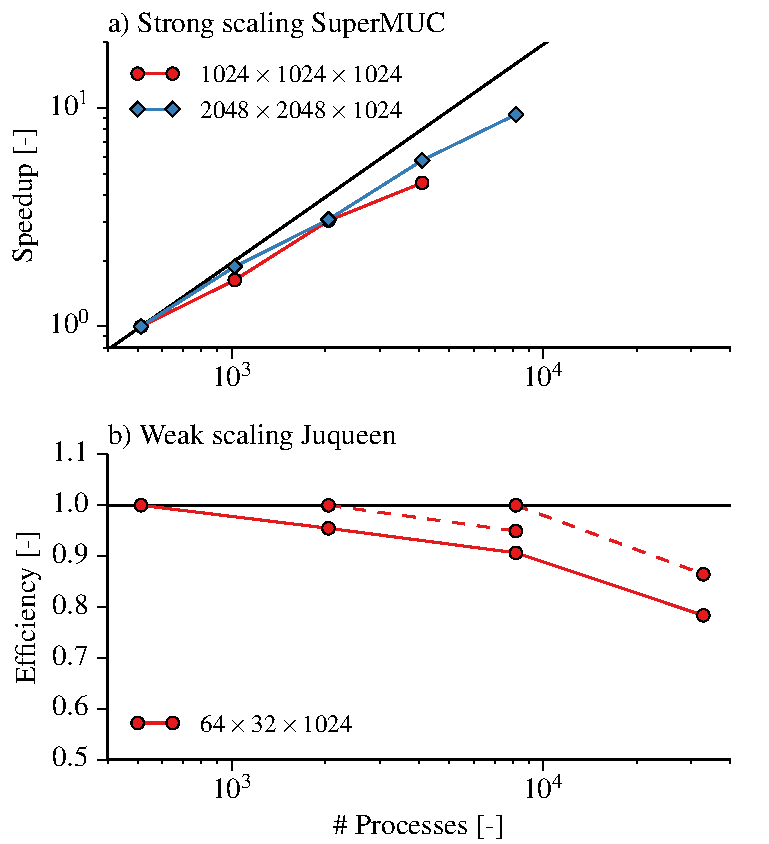
\includegraphics[width=8.3cm]{figs/scaling.pdf}
\end{center}
\caption{Error convergence of the spatial discretization in the two-dimensional Taylor-Green vortex. The dashed black line shows second-order convergence, the dotted black line shows fourth-order convergence.}
\end{figure}

\section{Performance GPU (CUDA) implementation}

Comparison single NVIDIA Quadro K6000 (Cuda 6.5) versus Thunder cluster (2 Intel Xeon E5-2670 CPU's per node, 16 cores per node, Intel 15.01 with OpenMPI 1.8.4). Bomex case (Bxx), with grid dimensions of $64^3$, $128^3$, $256^3$ and $512^2 \times 384$. Moser180 and Moser600 default case from microhh repo. All cases without statistics. 

\begin{table}[t]
\caption{Performance relative to GPU}
\begin{tabular}{rccccc}
\tophline
case & $n$=1 & $n$=16 & $n$=32 & $n$=64   \\
\middlehline
B64  & 18.49 & 1.93 & 1.14 & 0.95 \\
B128 & 28.01 & 2.98 & 1.51 & 0.92 \\
B256 & 27.76 & 3.02 & 1.59 & 0.91 \\
B512 & 29.88 & 3.03 & 1.56 & 0.86 \\
\middlehline
M180 & 21.57 & 2.17 & 1.13 & 0.69 \\
M600 & 22.55 & 2.25 & 1.06 & 0.60 \\
\bottomhline
\end{tabular}
\end{table}

\section{Model evaluation}
\subsection{Evaluation of the dynamical core}
\subsubsection{Taylor-Green vortex}
Bla.
\begin{figure}[t]
\vspace*{2mm}
\begin{center}
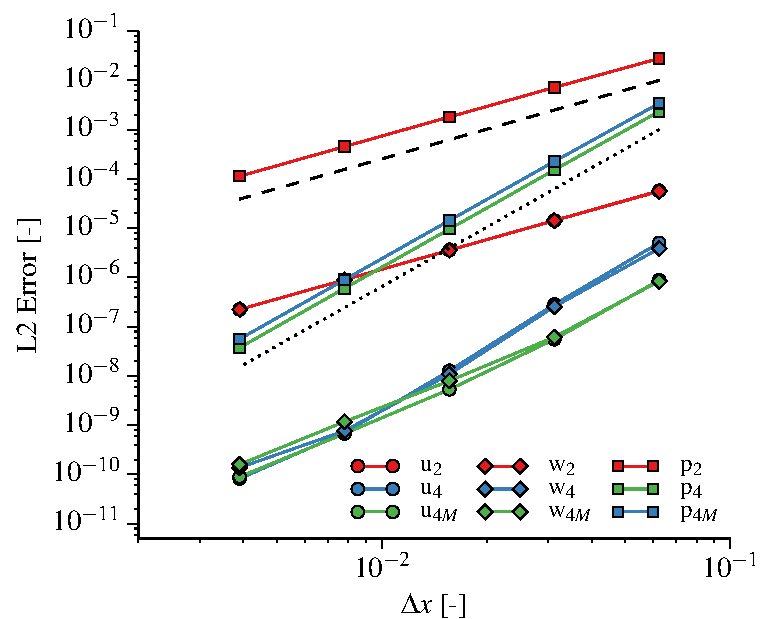
\includegraphics[width=8.3cm]{figs/taylorgreen.pdf}
\end{center}
\caption{Error convergence of the spatial discretization in the two-dimensional Taylor-Green vortex. The dashed black line shows second-order convergence, the dotted black line shows fourth-order convergence.}
\end{figure}

\subsubsection{Energy conservation and time accuracy}\label{sec:validationtime}
Bla.
\begin{figure}[t]
\vspace*{2mm}
\begin{center}
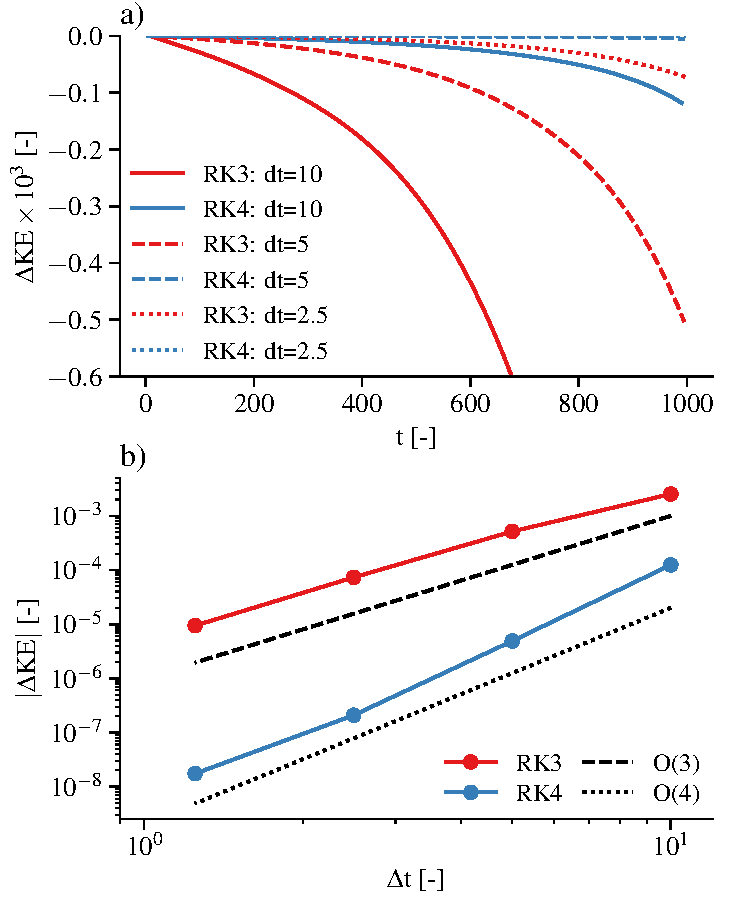
\includegraphics[width=8.3cm]{figs/timeconvergence.pdf}
\end{center}
\caption{Time evolution of the energy loss during 1000 time units of random noise advection for the RK3 and RK4 time integration schemes for three different time steps (a), and error convergence of the temporal discretization for the RK3 and RK4 scheme (b).}
\end{figure}

\subsubsection{Laminar katabatic flow}

\subsection{Comparison against known case studies}

\subsubsection{Channel flow}
The first experiment we compare against data is a neutral channel flow as discussed in MOSER. Strictly speaking, this is an evaluation of the dynamical core of the model, but as the flow is turbulent, we cannot compare it against an analytical solution.

The simulation has a Reynolds-$\tau$ number of 590. SPECS

Figure \ref{fig:moser_velocity}a shows the normalized horizontally-averaged streamwise velocity in panel, and the normalized rms of all three velocity components in Figure \ref{fig:moser_velocity}b. All plotted variables show a perfect match with the data and are indistinguishable from Moser's data. In order to further assess the accuracy of the data, we show the budgets of the variances in Figure \ref{fig:moser_budget}. Also here, the match with the reference data is excellent, which indicates that the whole range of spatial scales in the flow is represented well and that the fourth-order scheme is well able to pick up the details of for instance the disspiation $\epsilon$ that depends on local gradients in the flow.

The findings in the previous paragraph are further corroborated by the spectra shown in Figure \ref{fig:moser_spectra}.  

\begin{figure}[t]
\vspace*{2mm}
\begin{center}
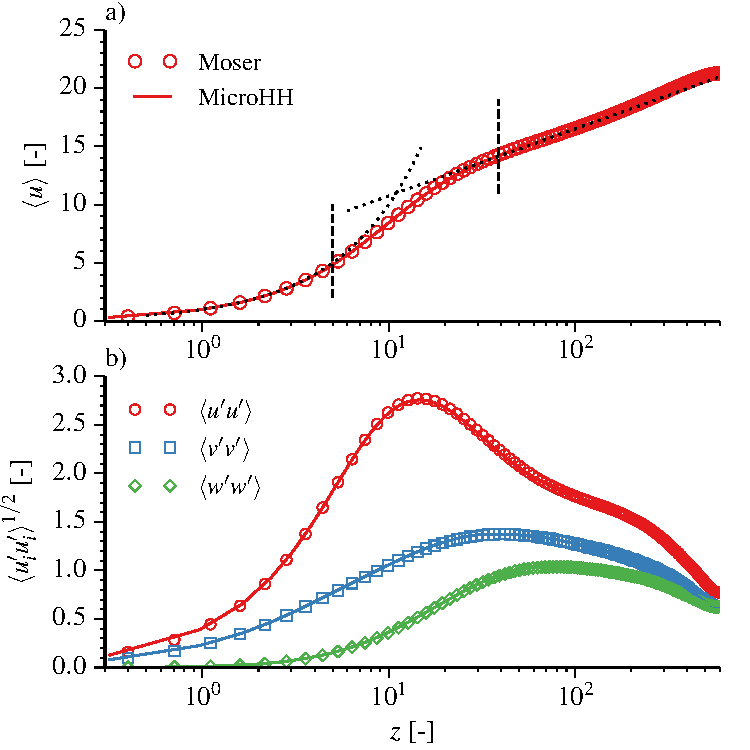
\includegraphics[width=8.3cm]{figs/gmd_m590_umean_var.pdf}
\end{center}
\caption{Moser590. Dashed line = spectra location. $z$ normalized with $u_\tau / \nu$, velocities with $u_\tau^{-1}$.}\label{fig:moser_velocity}
\end{figure}

%% TWO-COLUMN FIGURES
\begin{figure*}[t]
\vspace*{2mm}
\begin{center}
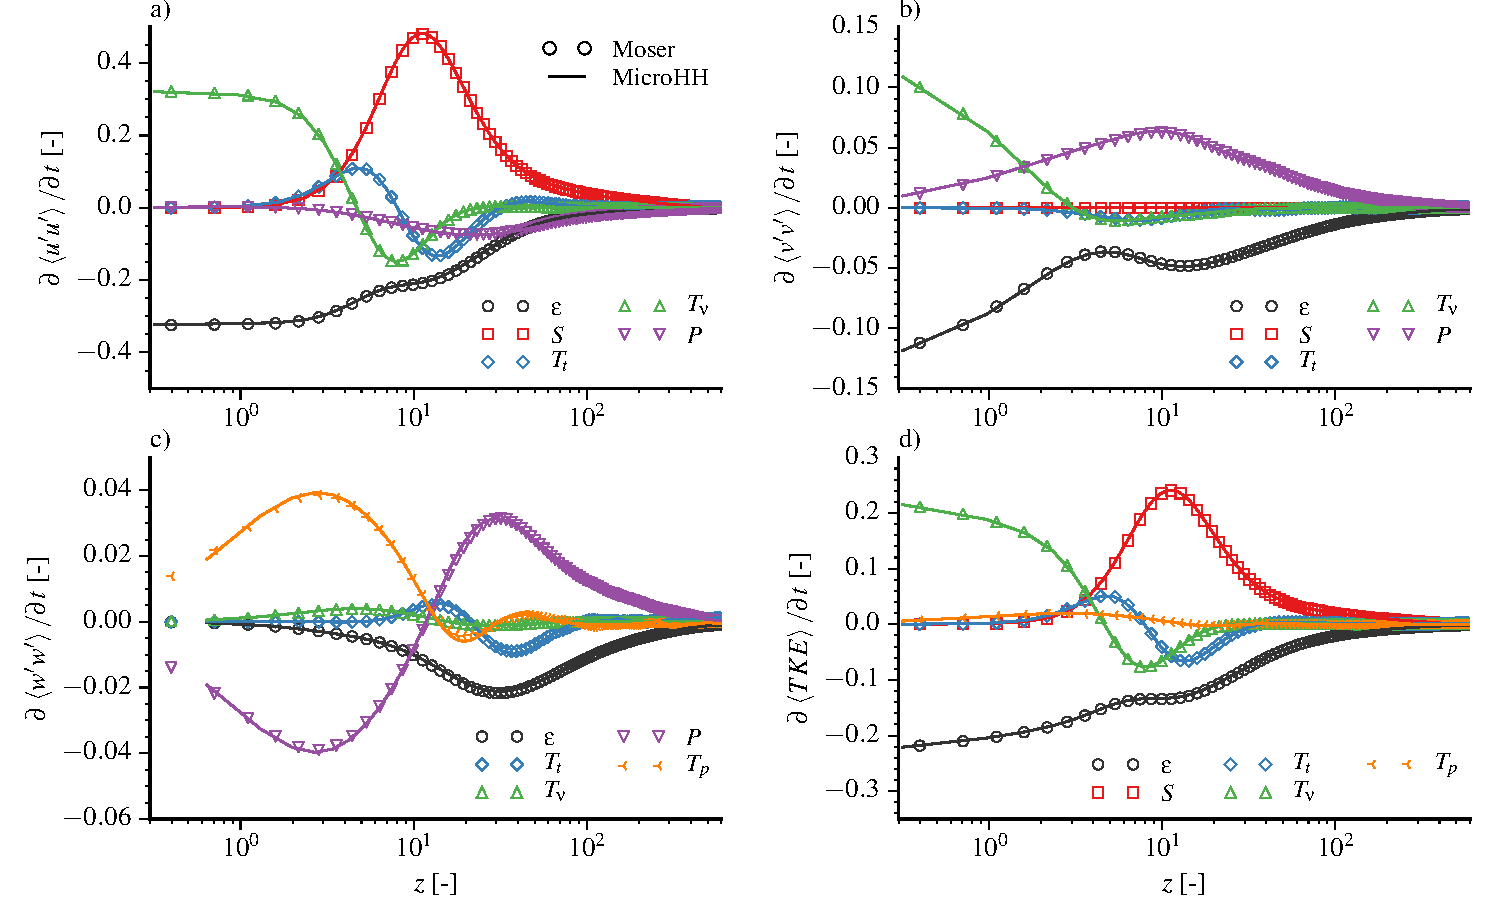
\includegraphics[width=16.6cm]{figs/gmd_m590_turb_budg.pdf}
\end{center}
\caption{Moser590 variance and TKE budgets. $z$ normalized with $u_\tau / \nu$, variances and TKE budget with $\nu / u_\tau^{4}$.}\label{fig:moser_variance}
\end{figure*}

%% TWO-COLUMN FIGURES
\begin{figure*}[t]
\vspace*{2mm}
\begin{center}
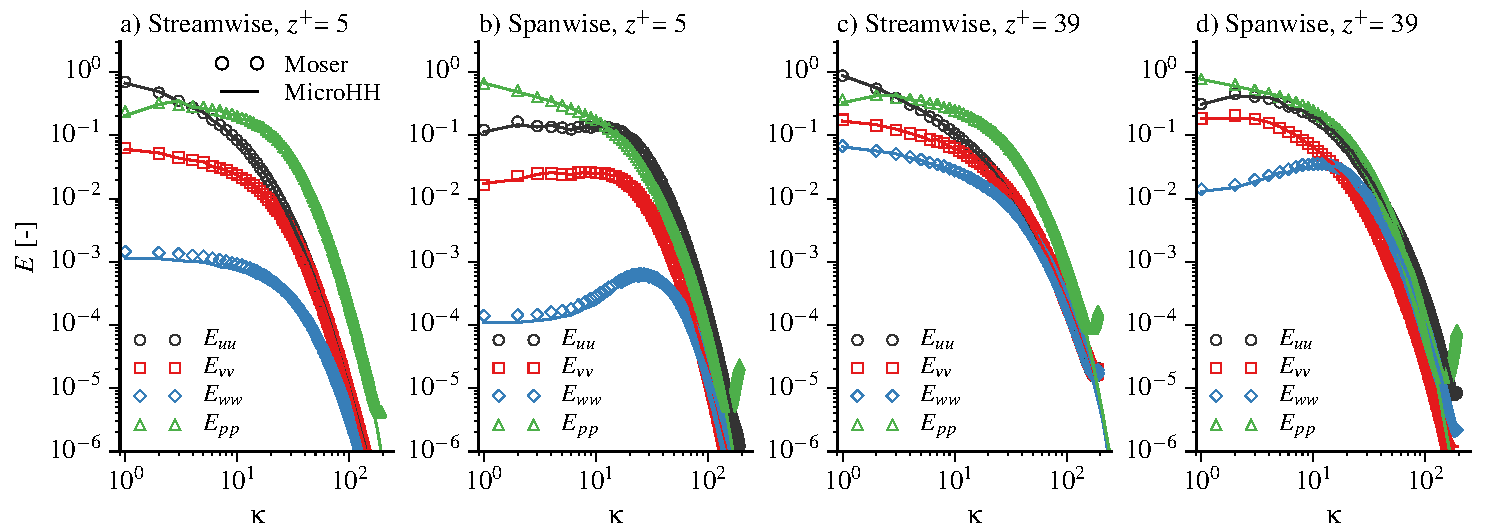
\includegraphics[width=16.6cm]{figs/gmd_m590_spectra_4x1.pdf}\label{fig:moser_spectra}
\end{center}
\caption{Moser590 spectra, velocity spectra are normalized with $u_\tau^{-2}$, pressure spectra with $u_\tau^{-4}$}
\end{figure*}

\subsubsection{Dry CBL}
\subsubsection{Bomex}

%% TWO-COLUMN FIGURES
\begin{figure*}[t]
\vspace*{2mm}
\begin{center}
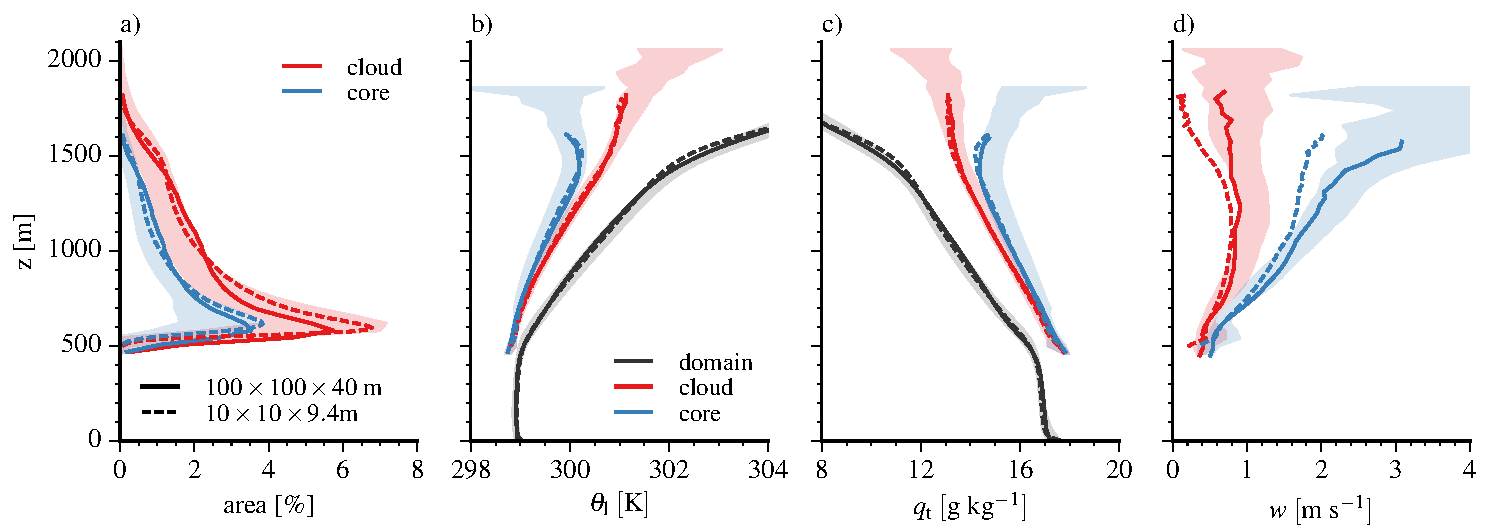
\includegraphics[width=16.6cm]{figs/gmd_bomex_profs.pdf}
\end{center}
\caption{BOMEX, averaged over hour 5-6, shading = average Siebesma +/- 1 stddev.}
\end{figure*}
`

\subsubsection{ARM}
\subsubsection{GABLS1}

\begin{figure*}[t]
\vspace*{2mm}
\begin{center}
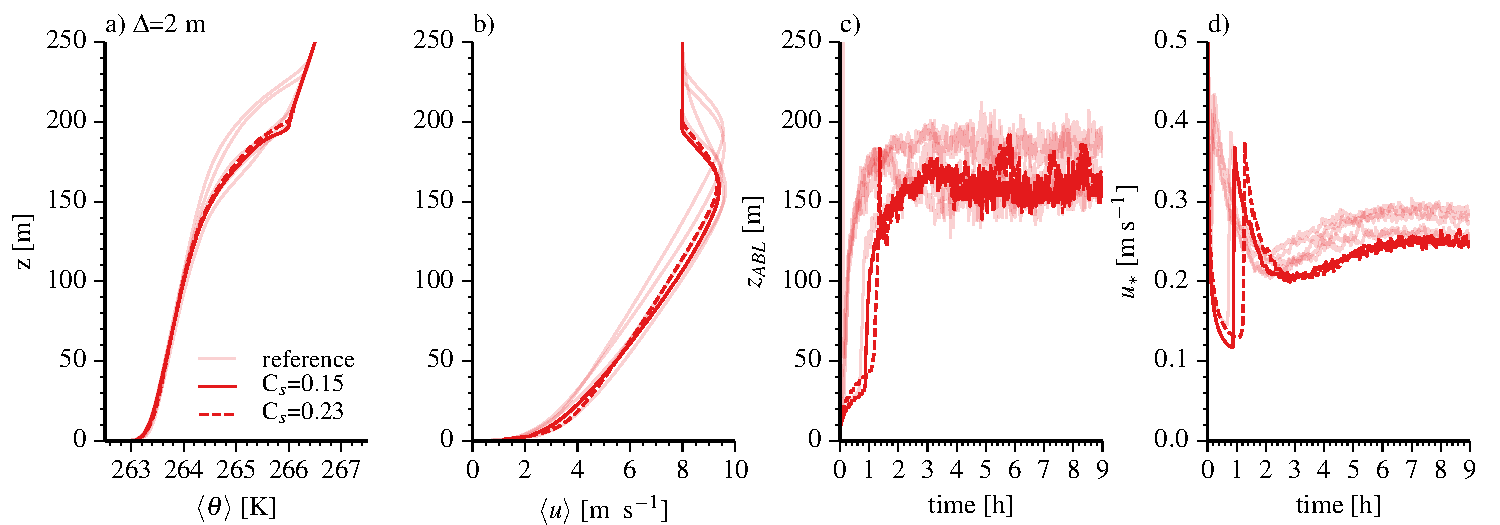
\includegraphics[width=16.6cm]{figs/gmd_gabls_prof_tser.pdf}
\end{center}
\caption{GABLS1 profiles}
\end{figure*}

%\begin{figure}[t]
%\vspace*{2mm}
%\begin{center}
%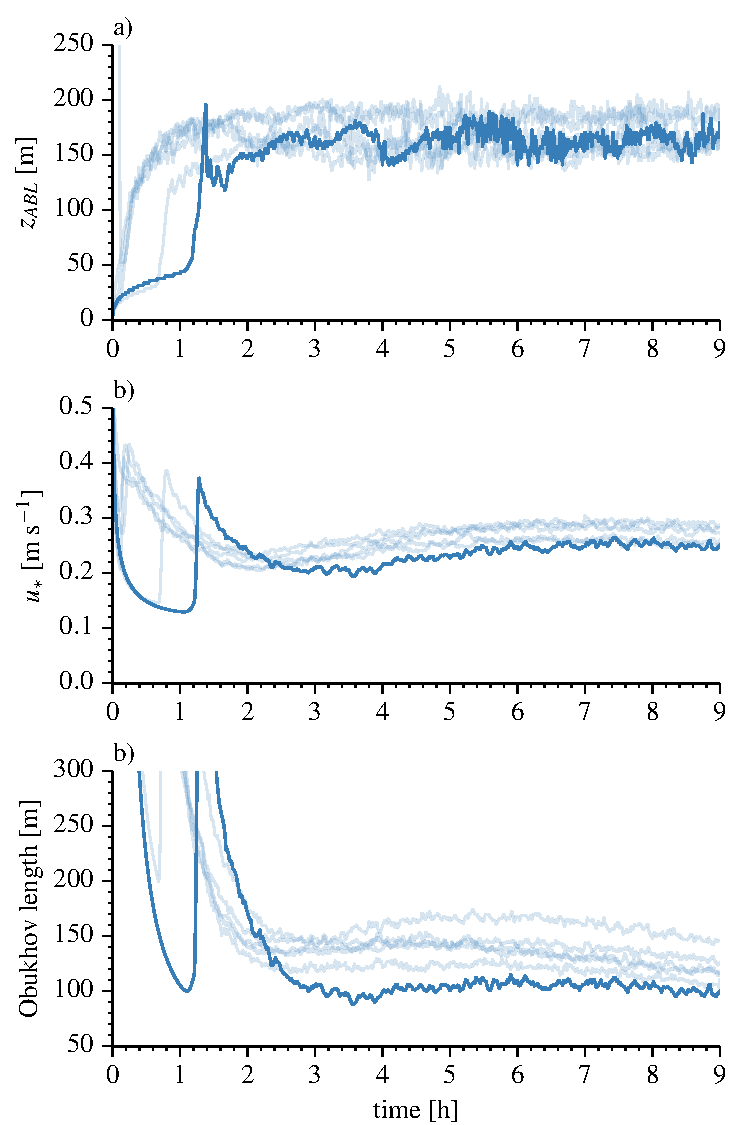
\includegraphics[width=8.3cm]{figs/gmd_gabls_tser.pdf}
%\end{center}
%\caption{GABLS1 time series}
%\end{figure}

\subsubsection{Katabatic flow}
\subsubsection{Governing equations}

\noindent Katabatic flow (wind) is an atmospheric buoyantly driven boundary-layer flow along a cooled sloping surface in a stratified fluid. We simulate a particular case of katabatic wind that blows along a planar, doubly-infinite slope with the surface cooling prescribed in terms of a spatially and temporally constant surface heat/buoyancy flux. Effects of the Earth rotation on the katabatic wind are neglected, which corresponds to the assumption of a very large Rossby number, and the diffusivities for momentum and temperature are taken equal each other (Prandtl number is assumed to be 1). 

Momentum balance equations for a katabatic flow in the Boussinesq approximation are the following (Fedorovich and Shapiro 2009): 
\begin{eqnarray} \label{GrindEQ__1_} 
\nonumber \frac{\partial u}{\partial t} +u\frac{\partial u}{\partial x} +v\frac{\partial u}{\partial y} +w\frac{\partial u}{\partial z} =-\frac{\partial \pi }{\partial x} +\beta \theta \sin \alpha \\ +\nu \left(\frac{\partial ^{2} u}{\partial x^{2} } +\frac{\partial ^{2} u}{\partial y^{2} } +\frac{\partial ^{2} u}{\partial z^{2} } \right),  
\end{eqnarray} 
\begin{eqnarray} \label{GrindEQ__2_} 
\nonumber \frac{\partial v}{\partial t} +u\frac{\partial v}{\partial x} +v\frac{\partial v}{\partial y} +w\frac{\partial v}{\partial z} =-\frac{\partial \pi }{\partial y} \\+\nu \left(\frac{\partial ^{2} v}{\partial x^{2} } +\frac{\partial ^{2} v}{\partial y^{2} } +\frac{\partial ^{2} v}{\partial z^{2} } \right),  
\end{eqnarray} 
\begin{eqnarray} \label{GrindEQ__3_} 
\nonumber \frac{\partial w}{\partial t} +u\frac{\partial w}{\partial x} +v\frac{\partial w}{\partial y} +w\frac{\partial w}{\partial z} =-\frac{\partial \pi }{\partial z} +\beta \theta \cos \alpha \\ +\nu \left(\frac{\partial ^{2} w}{\partial x^{2} } +\frac{\partial ^{2} w}{\partial y^{2} } +\frac{\partial ^{2} w}{\partial z^{2} } \right),  
\end{eqnarray} 
with the heat balance given by
\begin{eqnarray} \label{GrindEQ__4_} 
\nonumber \frac{\partial \theta }{\partial t} +u\frac{\partial \theta }{\partial x} +v\frac{\partial \theta }{\partial y} + w\frac{\partial \theta }{\partial z} =-\gamma (u\sin \alpha +w\cos \alpha ) \\+ \nu \left(\frac{\partial ^{2} \theta }{\partial x^{2} } + \frac{\partial ^{2} \theta }{\partial y^{2} } + \frac{\partial ^{2} \theta }{\partial z^{2} } \right),
\end{eqnarray}

and mass conservation represented by the continuity equation for an incompressible fluid,
\begin{equation} \label{GrindEQ__5_} 
\frac{\partial u}{\partial x} +\frac{\partial v}{\partial y} +\frac{\partial w}{\partial z} =0.  
\end{equation}
 
\noindent  In the above equations, $u,{\rm \; }v,{\rm \; }w$ are velocity components in the right-hand slope-following Cartesian coordinate system (see Fig.~\ref{Figure_coord}) with $x$, $y$, and $z$ being the upslope, cross-slope, and slope-normal coordinates, respectively, $\pi =[p-p_{e} (z')]/\rho _{r} $ is the normalized pressure perturbation [$p_{e} (z')$ is the environmental pressure, $z'$ is the true vertical coordinate, $\rho _{r} $=const is the reference density value], $\theta =\Theta -\Theta _{e} (z')$ is the potential temperature perturbation, $\gamma =d\Theta _{e} /dz'$=const is the gradient of environmental potential temperature, $\beta =g/\Theta _{r} $ is the buoyancy parameter ($\Theta _{r} $=const is the reference potential temperature value, \textit{g} is the gravitational acceleration), $\alpha $ is the slope angle, $\nu $ is the kinematic viscosity equal to the thermal diffusivity.

\begin{figure}
\centerline{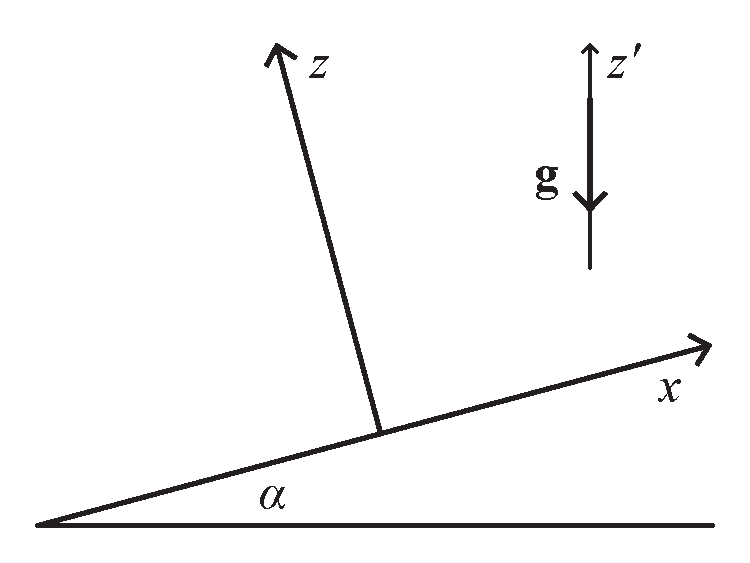
\includegraphics[width=8.3cm]{figs/Figure_coord.pdf}}
\caption{Schematic of the slope-following coordinate system used in simulations of katabatic flows.}
\label{Figure_coord}
\end{figure}

The heat balance equation \eqref{GrindEQ__4_} may be conveniently rewritten in terms of the buoyancy $b\equiv \beta \theta $ as
\begin{eqnarray} \label{GrindEQ__6_} 
\nonumber \frac{\partial b}{\partial t} +u\frac{\partial b}{\partial x} +v\frac{\partial b}{\partial y} +w\frac{\partial b}{\partial z} =-N^{2} (u\sin \alpha +w\cos \alpha )\\+\nu \left(\frac{\partial ^{2} b}{\partial x^{2} } +\frac{\partial ^{2} b}{\partial y^{2} } +\frac{\partial ^{2} b}{\partial z^{2} } \right),  
\end{eqnarray} 

\noindent  where $N=(\beta \gamma )^{1/2} $ is the Brunt-V\"{a}is\"{a}l\"{a} (or buoyancy) frequency.

The lateral boundary conditions for prognostic variables (\textit{u}, \textit{v}, \textit{w}, \textit{b}) and normalized pressure $\pi $ are periodic (the sloping surface is supposed to be doubly infinite along \textit{x} and \textit{y}). The upper boundary conditions (large \textit{z}) are $\partial \varphi /\partial z=0$, where $\varphi $ is any of (\textit{u}, \textit{v}, \textit{w}, \textit{b}), and $\partial \pi /\partial z$ is obtained from \eqref{GrindEQ__3_}. The surface (\textit{z}=0) conditions are no-slip and impermeability (\textit{u}=\textit{v}=\textit{w}=0), with $\partial \pi /\partial z$ obtained from \eqref{GrindEQ__3_}, and $\nu (\partial b/\partial z)=-B_{s} $, where $B_{s} $ is the surface buoyancy flux which also has a meaning of the surface energy production rate.

Results of numerical simulations of the turbulent katabatic flow based on the complete set of governing equations \eqref{GrindEQ__1_} - \eqref{GrindEQ__3_}, \eqref{GrindEQ__5_}, \eqref{GrindEQ__6_} are presented in section 2.

An early milestone in the formal description of katabatic flows was the Prandtl (1942) one-dimensional model for the laminar flow of a viscous stably-stratified fluid along a uniformly cooled sloping surface. In the Prandlt model, the along-slope advection of environmental (mean) temperature balances thermal diffusion, and the along-slope component of buoyancy balances diffusion of along-slope momentum. All other terms in the equations of motion and thermodynamic energy are identically zero, which provides
\begin{equation} \label{GrindEQ__7_} 
b\sin \alpha +\nu \frac{\partial ^{2} u}{\partial z^{2} } =0,  
\end{equation} 
\begin{equation} \label{GrindEQ__8_} 
-N^{2} u\sin \alpha +\nu \frac{\partial ^{2} b}{\partial z^{2} } =0,  
\end{equation} 

\noindent  with the following boundary conditions: $u(0)=0$, $b(0)=b_{s} $ or $\left. -\nu (db/dz)\right|_{z=0} =B_{s} $, and $u\to 0$ and $b\to 0$ as $z\to \infty $. The controlling parameters of the reduced  (Prandtl) problem are $\alpha $, $\nu $, $N$, and either $b_{s} $ or $B_{s} $.  The original solution was obtained by Prandtl for the flow with prescribed surface buoyancy. Here, however, we focus on the Prandtl-model solution for the flow driven by a constant negative surface buoyancy flux. This solution was obtained in Fedorovich and Shapiro (2009) based on the work of Shapiro and Fedorovich (2004). 

Introducing generic length ($L$), velocity ($V$), and buoyancy ($B$) scales, and applying these scales in \eqref{GrindEQ__7_} and \eqref{GrindEQ__8_}, we come to the following non-dimensionalized momentum and buoyancy balance equations of the Prandtl model:
\begin{equation} \label{GrindEQ__9_} 
b_{n} +\frac{\nu V}{L^{2} \sin \alpha B} \frac{\partial ^{2} u_{n} }{\partial z_{n} ^{2} } =0,  
\end{equation} 
\begin{equation} \label{GrindEQ__10_} 
-u_{n} +\frac{\nu B}{L^{2} \sin \alpha N^{2} V} \frac{\partial ^{2} b_{n} }{\partial z_{n} ^{2} } =0,  
\end{equation} 

\noindent with the boundary conditions transforming into $u_{n} (0)=0$, and $u_{n} \to 0$, $b_{n} \to 0$ as $z_{n} \to \infty $, and $\left. (db_{n} /dz_{n} )\right|_{z_{n} =0} =-\frac{B_{s} }{\nu } \frac{L}{B} $.

Defining the length, velocity, and buoyancy scales as
\begin{equation} \label{GrindEQ__11_}
L=\nu ^{1/2} N^{-1/2} \sin ^{-1/2} \alpha ,
\end{equation}
\begin{equation} \label{GrindEQ__12_}
V=\nu ^{-1/2} N^{-3/2} B_{s} \sin ^{-1/2} \alpha ,
\end{equation}
\begin{equation} \label{GrindEQ__13_}
B=\nu ^{-1/2} N^{-1/2} B_{s} \sin ^{-1/2} \alpha ,
\end{equation}
 
\noindent respectively, reduces the dimensionless problem \eqref{GrindEQ__9_}-\eqref{GrindEQ__10_} to
\begin{eqnarray} \label{GrindEQ__14_} 
b_{n} +\frac{\partial ^{2} u_{n} }{\partial z_{n} ^{2} } =0, \\-u_{n} +\frac{\partial ^{2} b_{n} }{\partial z_{n} ^{2} } =0,  
\end{eqnarray} 

\noindent where
\begin{equation} \label{GrindEQ__15_}
z_{n} =z\nu ^{-1/2} N^{1/2} \sin ^{1/2} \alpha ,
\end{equation}
\begin{equation} \label{GrindEQ__16_}
u_{n} =u\nu ^{1/2} N^{3/2} B_{s} ^{-1} \sin ^{1/2} \alpha ,
\end{equation}
\begin{equation} \label{GrindEQ__17_}
b_{n} =b\nu ^{1/2} N^{3/2} B_{s} ^{-1} \sin ^{1/2} \alpha ,
\end{equation}
 
\noindent with the boundary conditions $u_{n} (0)=0$, $\left. (db_{n} /dz_{n} )\right|_{z_{n} =0} =-1$, and $u_{n} \to 0$, $b_{n} \to 0$ as $z_{n} \to \infty $.

Equations \eqref{GrindEQ__14_} have the following analytical solutions (Shapiro and Fedorovich 2004):
\begin{eqnarray} \label{GrindEQ__18_} 
u_{n} =\sqrt{2} \sin (z_{n} /\sqrt{2} )\exp (-z_{n} /\sqrt{2} ),\\b_{n} =\sqrt{2} \cos (z_{n} /\sqrt{2} )\exp (-z_{n} /\sqrt{2} ).  
\end{eqnarray} 


\noindent These solutions were employed for evaluation of the numerical predictions of velocity and buoyancy profiles in a Prandtl-type laminar katabatic flow. Results of the evaluation are presented in section 3.

\section{Turbulent katabatic flow}
\smallskip

\subsection{Simulation settings}
\smallskip
\begin{itemize}
  \setlength{\itemsep}{0pt}
  \setlength{\parskip}{0pt}
  \setlength{\parsep}{0pt}  
  \item Slope angle: $\alpha = 60^{\circ}$
  \item Surface buoyancy flux: $B_{s} $ = $-0.5{\rm\, m}^{\rm 2}\, {\rm s}^{{\rm -3}} $
  \item Brunt-V\"{a}is\"{a}l\"{a} (buoyancy) frequency: $N$ = $1\,{\rm s}^{{\rm -1}}$
  \item Kinematic viscosity/thermal diffusivity:\\$\nu$ = $-0.0001{\rm\, m}^{\rm 2}\, {\rm s}^{{\rm -1}} $
  \item Domain size: ($X{\times}Y{\times}Z$) = 0.64${\rm\, m}\times$0.64${\rm\, m}\times$1.6${\rm\, m}$
  \item Numerical grid dimensions: \\($n_x{\times}n_y{\times}n_z$) = $256 \times 256 \times 640$
  \item Grid structure: uniform (non-stretched) grid in all three directions, with $\Delta x = \Delta y = \Delta z$ = 0.0025${\rm\, m}$
  \item Time step: adaptive
  \item Initial condition: stratified fluid at rest above the slope with zero surface buoyancy flux
  \item Lateral boundary conditions: periodic
  \item Lower boundary conditions: no-slip and impermeability conditions for velocity, surface-flux condition for buoyancy
  \item Upper boundary conditions: free-slip conditions for velocity, zero-gradient condition for buoyancy
\end{itemize}
\subsection{Flow description and simulation results}

Motion starts once the buoyancy flux is applied at the sloping surface. After passing through relatively short transition stage, the flow becomes turbulent. It is characterized  by random, large-amplitude fluctuations of velocity and buoyancy fields in the near-slope core region and shows a quasi-periodic oscillatory behavior at larger distances from the slope. A typical duration of the transition stage in the conducted simulations is about several seconds. Mean profiles of along-slope velocity component  and buoyancy as well as profiles of second-order turbulence statistics, such as kinematic turbulent fluxes of momentum and buoyancy, and velocity-component and buoyancy fluctuation variances, were evaluated by averaging  the simulated flow fields spatially over $X-Y$ planes and temporally over five oscillation periods beyond the transition stage.

For comparison, the same katabatic flow case was reproduced using the numerical code (hereafter referred to FS09) that was employed to simulate turbulent slope flows in Shapiro and Fedorovich (2008) and Fedorovich and Shapiro (2009). In the version of the code used in this comparison study, the time advancement was performed with an Asselin-filtered second-order leapfrog scheme (Durran 1999). The spatial derivatives were approximated by second-order finite-difference expressions on a staggered uniform grid. The Poisson equation for pressure was solved with a fast Fourier transform technique over the $X-Y$ planes and a tri-diagonal matrix inversion method in the slope-normal direction. No-slip and impermeability conditions are applied on the velocity field at the slope surface. Equation \eqref{GrindEQ__3_} was used to formulate a Neumann boundary condition for the pressure at the surface and at the outer boundary of the domain (large $z$). Normal gradients of prognostic variables (velocity components and buoyancy) are set to zero at the outer computational boundary, and periodic boundary conditions are imposed at the $X-Z$ and $Y-Z$ boundaries of the computational domain.

Numerical results obtained with both numerical codes testify that stable environmental stratification in combination with negative surface buoyancy forcing in the katabatic flow leads to an effective suppression of vertical turbulent exchange in the flow region adjacent to the slope. This suppression results in a shallow near-surface sublayer with strong buoyancy gradients (Fig.~\ref{katabatic_b}) capped by a narrow mean-velocity jet with peak velocity located very close to the ground. (Fig.~\ref{katabatic_u}).

\begin{figure}
\centerline{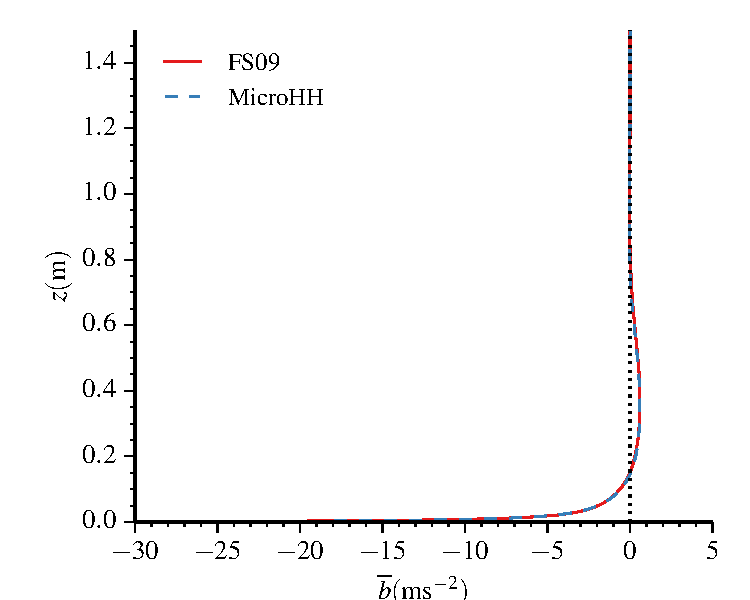
\includegraphics[width=8.3cm]{figs/katabatic_b.pdf}}
\caption{Profile of the mean buoyancy as predicted by MicroHH and FS09.}
\label{katabatic_b}
\end{figure}
 
\begin{figure}
\centerline{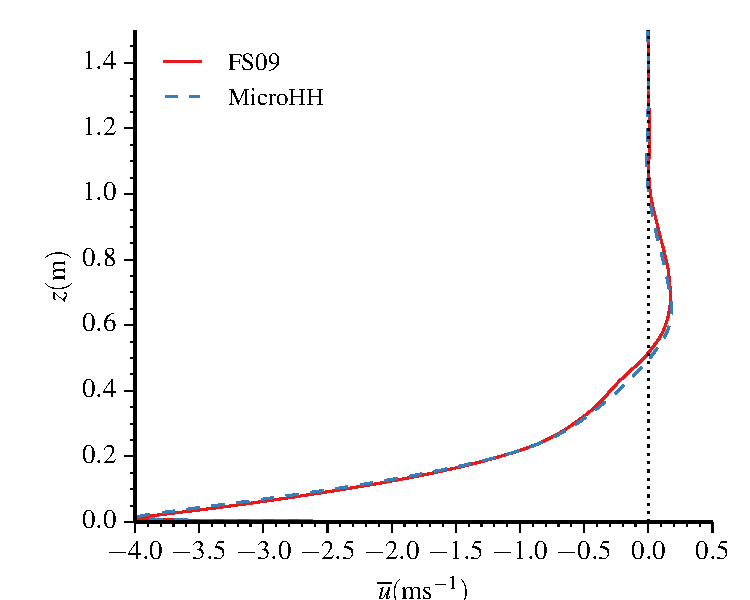
\includegraphics[width=8.3cm]{figs/katabatic_u.pdf}}
\caption{Profile of the mean along-slope velocity as predicted by MicroHH and FS09.}
\label{katabatic_u}
\end{figure}

As revealed by the buoyancy variance profiles in (Fig.~\ref{katabatic_bb}), the buoyancy fluctuations in the simulated katabatic flow attain their maximum magnitude extremely close to the wall, roughly within the region where maximum gradients are observed in the mean buoyancy profiles (Fig.~\ref{katabatic_b}). The drop of $\overline{b'b'}$ beyond the maximum is also rather sharp which means that significant fluctuations of the buoyancy are restricted to a comparatively thin near-wall sublayer.

\begin{figure}
\centerline{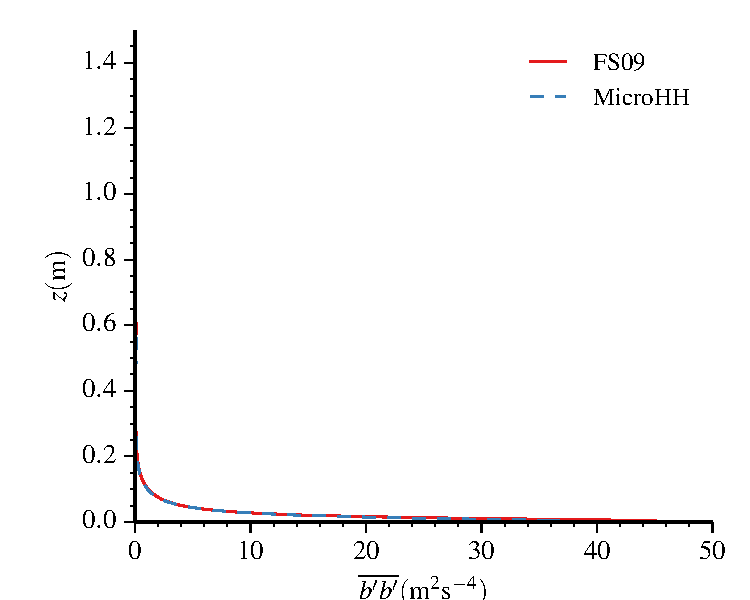
\includegraphics[width=8.3cm]{figs/katabatic_bb.pdf}}
\caption{Profile of the buoyancy variance as predicted by MicroHH and FS09.}
\label{katabatic_bb}
\end{figure}

Along-slope velocity fluctuations of notable magnitudes are distributed over the layer that is about four times thicker than the layer which contains most of the buoyancy variance (compare Fig.~\ref{katabatic_uu} and Fig.~\ref{katabatic_bb}). While the two codes agree with respect to predicting the overall behavior of $\overline{u'u'}$, MicroHH predicts a smoother and stronger maximum of the velocity variance than FS09. The magnitudes of the maxima, though, are fairly close to each other in Fig.~\ref{katabatic_uu}.

\begin{figure}
\centerline{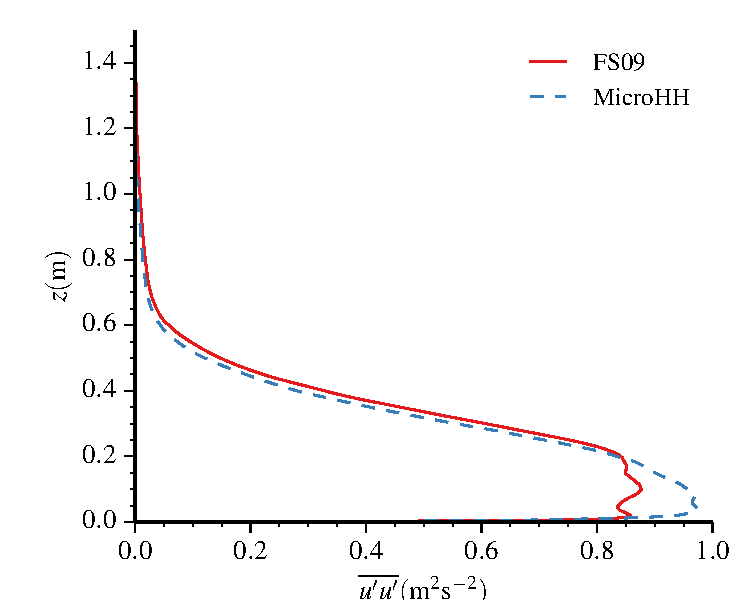
\includegraphics[width=8.3cm]{figs/katabatic_uu.pdf}}
\caption{Profile of the along-slope velocity variance as predicted by MicroHH and FS09.}
\label{katabatic_uu}
\end{figure}

Comparisons of profiles of the cross-slope velocity component variance, $\overline{v'v'}$, and the slope-normal component variance, $\overline{w'w'}$, are presented in Fig.~\ref{katabatic_vv} and Fig.~\ref{katabatic_ww}, respectively.

\begin{figure}
\centerline{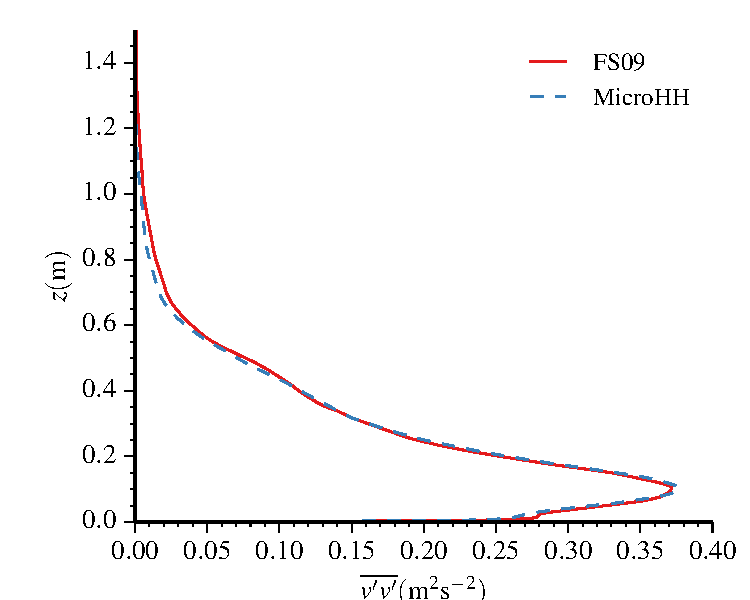
\includegraphics[width=8.3cm]{figs/katabatic_vv.pdf}}
\caption{Profile of the cross-slope velocity variance as predicted by MicroHH and FS09.}
\label{katabatic_vv}
\end{figure}

\begin{figure}
\centerline{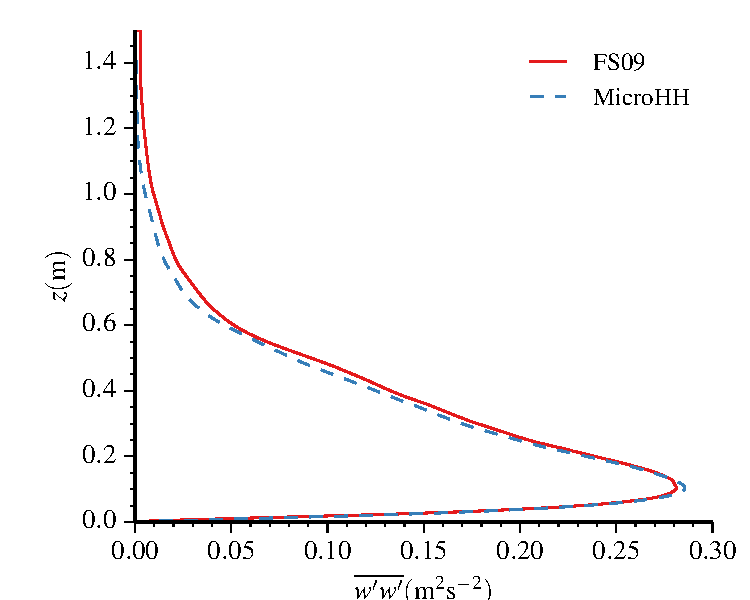
\includegraphics[width=8.3cm]{figs/katabatic_ww.pdf}}
\caption{Profile of the slope-normal velocity variance as predicted by MicroHH and FS09.}
\label{katabatic_ww}
\end{figure}

Profiles of slope-normal fluxes of momentum, $\overline{w'u'}$ (Fig.~\ref{katabatic_wu}), and buoyancy, $\overline{w'b'}$ (Fig.~\ref{katabatic_wb}), indicate that zero crossings in the mean profiles of \textit{b} and \textit{u} are closely co-located with the minima and maxima of the fluxes $\overline{u'w'}$ and $\overline{b'w'}$ except for locations very close to the wall, where molecular effects are important. Typically, molecular fluxes in the simulated flows become negligible at distances from the surface that are significantly smaller than the elevation of the mean velocity maximum (jet elevation).

\begin{figure}
\centerline{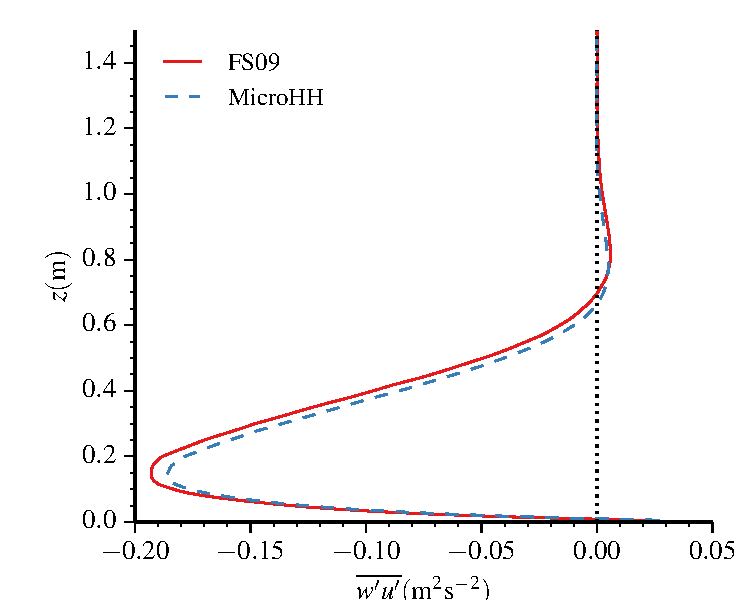
\includegraphics[width=8.3cm]{figs/katabatic_wu.pdf}}
\caption{Profile of the slope-normal turbulent kinematic momentum flux as predicted by MicroHH and FS09.}
\label{katabatic_wu}
\end{figure}
 
\begin{figure}
\centerline{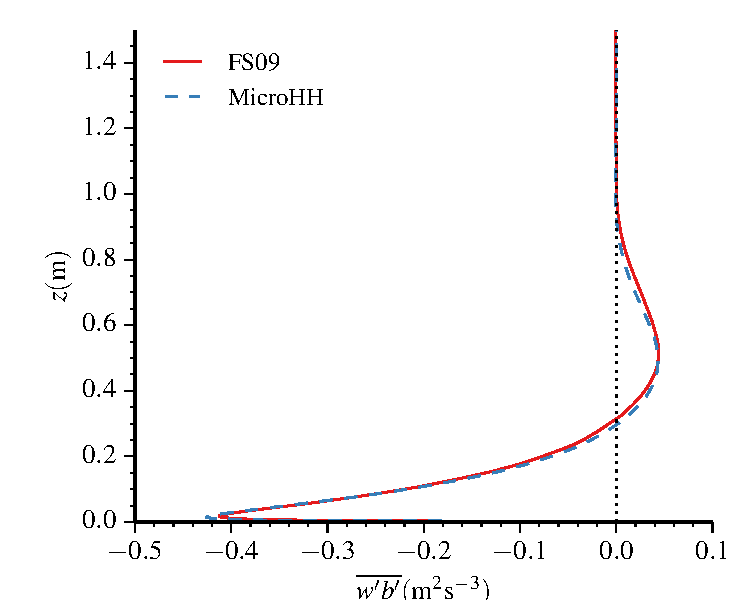
\includegraphics[width=8.3cm]{figs/katabatic_wb.pdf}}
\caption{Profile of the slope-normal turbulent kinematic buoyancy flux as predicted by MicroHH and FS09.}
\label{katabatic_wb}
\end{figure}

Flux profiles shown in Fig.~\ref{katabatic_wu} and Fig.~\ref{katabatic_wb} indicate that there is no region in the flow domain with constancy (even approximate) of either flux with distance from the wall. In more conventional boundary-layer type flows, the existence of height intervals with slowly changing (in the first approximation, constant) momentum and buoyancy fluxes is used as a foundation for similarity analyses and scalings. Such a constant-flux formalism does not apply, at least in a straightforward manner, to the considered katabatic flow case.

\section{Laminar katabatic flow}

\subsection{Simulation settings}

\begin{itemize}
  
  \setlength{\itemsep}{0pt}
  \setlength{\parskip}{0pt}
  \setlength{\parsep}{0pt} 
  \item Slope angle: $\alpha = 30^{\circ}$
  \item Surface buoyancy flux: $B_{s} $ = $-0.005{\rm\, m}^{\rm 2}\, {\rm s}^{{\rm -3}} $
  \item Brunt-V\"{a}is\"{a}l\"{a} (buoyancy) frequency: $N$ = $1\,{\rm s}^{{\rm -1}}$
  \item Kinematic viscosity/thermal diffusivity: \\$\nu$ = $-0.0005{\rm\, m}^{\rm 2}\, {\rm s}^{{\rm -1}} $
  \item Domain size: \\($X{\times}Y{\times}Z$) = 0.015625${\rm\, m}\times$0.001953${\rm\, m}\times$1${\rm\, m}$
  \item Numerical grid dimensions: ($n_x{\times}n_y{\times}n_z$) = $8 \times 1 \times 512$
  \item Grid structure: grid is stretched in the vertical ($z$), with near-surface $\Delta z$ = 0.001${\rm\, m}$, and uniform in $x$ direction  
  \item Time step: adaptive
  \item Initial condition: stratified fluid at rest above the slope with zero surface buoyancy flux
  \item Lateral boundary conditions: periodic
  \item Lower boundary conditions: no-slip and impermeability conditions for velocity, surface-flux condition for buoyancy
  \item Upper boundary conditions: free-slip conditions for velocity, zero-gradient condition for buoyancy
\end{itemize}

\subsection{Flow description and simulation results}

\begin{figure*}[t]
\vspace*{2mm}
\begin{center}
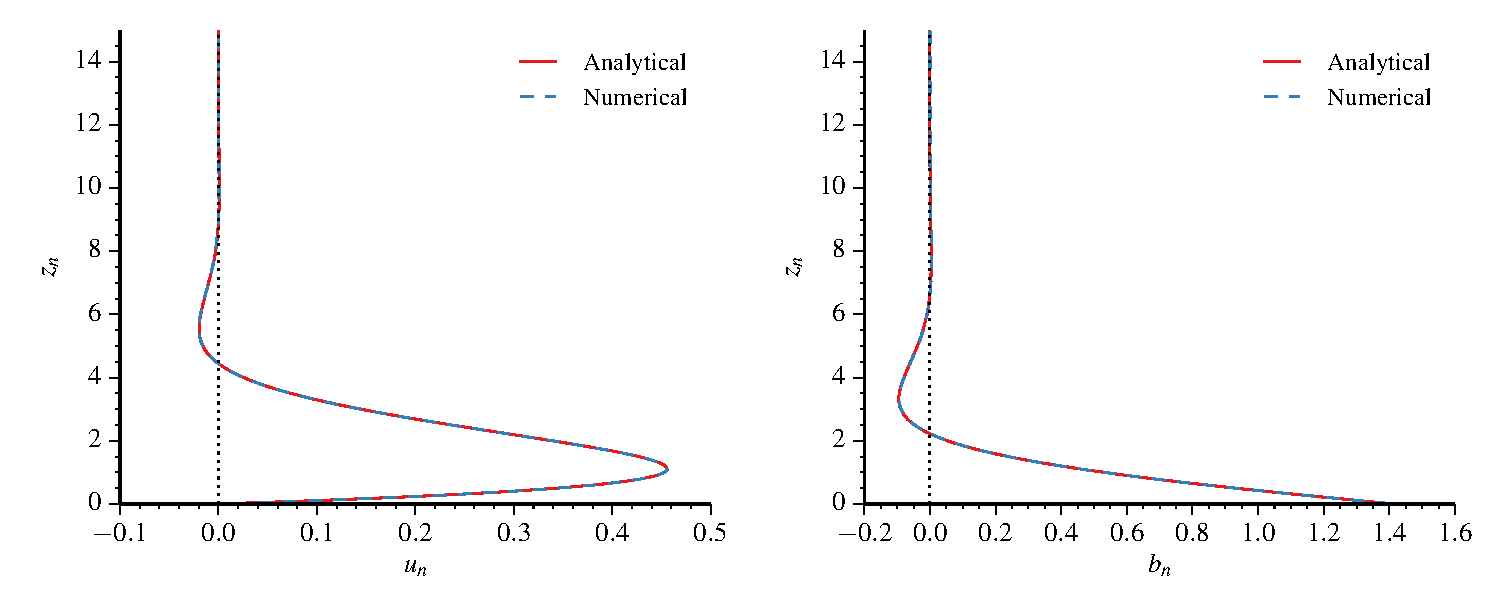
\includegraphics[width=16.6cm]{figs/prandtl.pdf}
\end{center}
\caption{Normalized numerical Prandtl-model solutions for velocity $u$ (left) and buoyancy $b$ (right) compared to their analytical counterparts.}
\label{prandtl}
\end{figure*}

After the negative buoyancy flux is applied at the surface, the fluid, which was initially at rest, goes through the series of decaying oscillations until it reaches the steady state corresponding to the Prandtl model solution. Numerical integration was performed sufficiently long for the oscillation amplitude to become a small fraction of the amplitude of the first oscillation. Computed steady-state profiles of along-slope velocity $u$ and buoyancy $b$ were averaged over $x$ and then normalized using scales \eqref{GrindEQ__11_} - \eqref{GrindEQ__13_}. Comparison of analytical and numerical solutions, which very closely agree with each other, is presented in Fig.~\ref{prandtl}.

\section{Future plans}
Currently, there are several ongoing projects to extend the model. The physical processes at are currenlty being implemented are microphysics and an interactive land surface model. [BART]

In parallel, preliminary experiments have been performed to include a Domain-Specific Language (DSL) that enables the expression of complex finite difference operators in a simple syntax. The project has shown great potential, for two reasons. First, the DSL reduces the chances of making errors, as the explicit indexing in computational kernels with spatial operators can be omitted. Second, the DSL allows for simple implementation of system specific tuning, such as loop tiling or OpenMP.

\conclusions  %% \conclusions[modified heading if necessary]
This paper has explained MicroHH, an new Computational Fluid Dynamics code for simulations of turbulent flows in the atmospheric boundary layer. 

\section{Availability of code and resources}
MicroHH has its own website at \url{http://microhh.org}. Its code is hosted at GitHub and can be accessed either via the website, or directly from 
\url{https://github.com/microhh/microhh}. A selection of visualizations can be viewed at the MicroHH channel at Vimeo \url{https://vimeo.com/channels/817195}.

\bibliographystyle{copernicus}
\bibliography{../../misc/refs}
\nopagebreak

\smallskip

\noindent Durran, D. R., 1999: \textit{Numerical Methods for Wave Equations in Geophysical Fluid Dynamics}, Springer-Verlag, New York, 465 pp.

\smallskip

\noindent Fedorovich, E., and A. Shapiro, 2009: Structure of numerically simulated katabatic and anabatic flows along steep slopes. \textit{Acta Geophysica},  \textbf{57}, 981-1010.

\smallskip

\noindent Prandtl, L., 1942: \textit{F\"{u}hrer durch die Str\"{o}mungslehre}, Vieweg und Sohn, Braunschweig, 382 pp.

\smallskip

\noindent Shapiro, A., and E. Fedorovich, 2004: Unsteady convectively driven flow along a vertical plate immersed in a stably stratified fluid. \textit{J. Fluid Mech}. \textbf{498}, 333-352.

\smallskip

\noindent Shapiro, A., and E. Fedorovich, 2008: Coriolis effects in homogeneous and inhomogeneous katabatic flows. \textit{Q. J. R. Meteorol. Soc.}, \textbf{134}, 353-370.
\end{document}
